\subsection{Explicación formal del problema}

Sea una matriz $M$ $\in$ $\mathbb{R}^{n \times m}$, donde cada posición de la matriz $M_{ij}$ tiene un valor asociado $h_{ij}$. El problema consiste en calcular el camino mínimo de casilleros desde la posición (1,1) hasta la posición ($N$,$M$), donde los únicos dos  movimientos posibles son:

\emph{Moverse hacia el casillero de abajo}: \[M_{i,j} \rightarrow M_{i+1,j}\] 

ó \emph{Moverse hacia el casillero de la derecha}: \[M_{i,j} \rightarrow M_{i,j+1}\]

Realizar estos movimientos tiene un costo que depende de un parámetro de entrada $H$:

\begin{equation} \label{costoHaciaAbajo}
   Costo(M_{i,j} \rightarrow M_{i+1,j}) = \left\{ 
     \begin{array}{lr}
       0 							& $ si $  |h_{i,j} - h_{i+1,j}| \leq H \\
       |h_{i,j} - h_{i+1,j}| - H 	&   $ caso contrario $ \\
     \end{array}
   \right.
\end{equation} 

\begin{equation}\label{costoHaciaDerecha}
  Costo(M_{i,j} \rightarrow M_{i,j+1}) = \left\{ 
     \begin{array}{lr}
       0 							& $ si $  |h_{i,j} - h_{i,j+1}| \leq H \\
       |h_{i,j} - h_{i,j+1}| - H 	&   $ caso contrario $ \\
     \end{array}
   \right.
\end{equation} 

\subsubsection{Ejemplos}

\begin{figure}[H]
\centering
\begin{minipage}{0.3\textwidth}
  \centering
    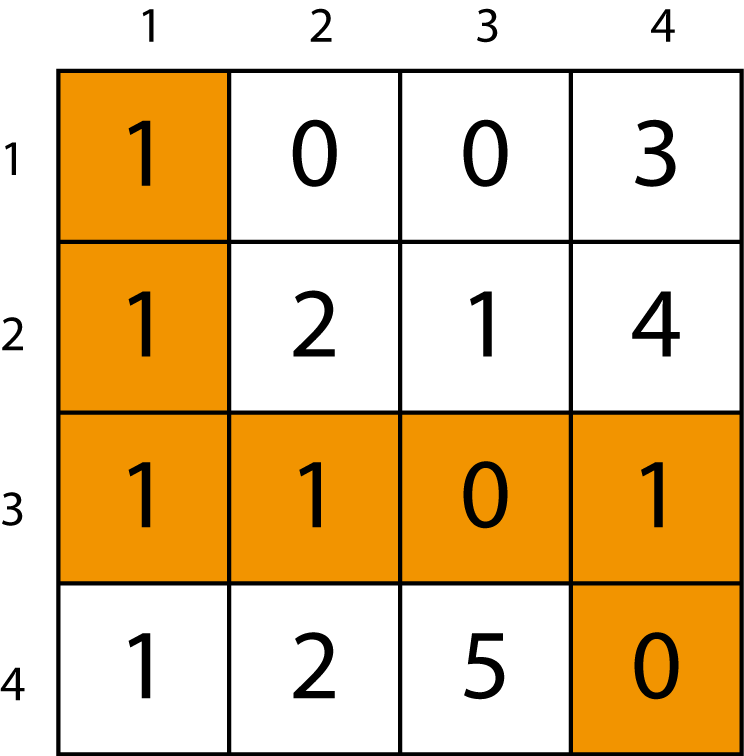
\includegraphics[width=1\textwidth]{img/3-1.png}
  \caption*{\footnotesize Ejemplo con H=0. El costo del camino mínimo resultante es 3.}
  \label{fig:3-1}
\end{minipage}%
\hspace{0.2\textwidth}
\begin{minipage}{0.3\textwidth}   
  \centering
    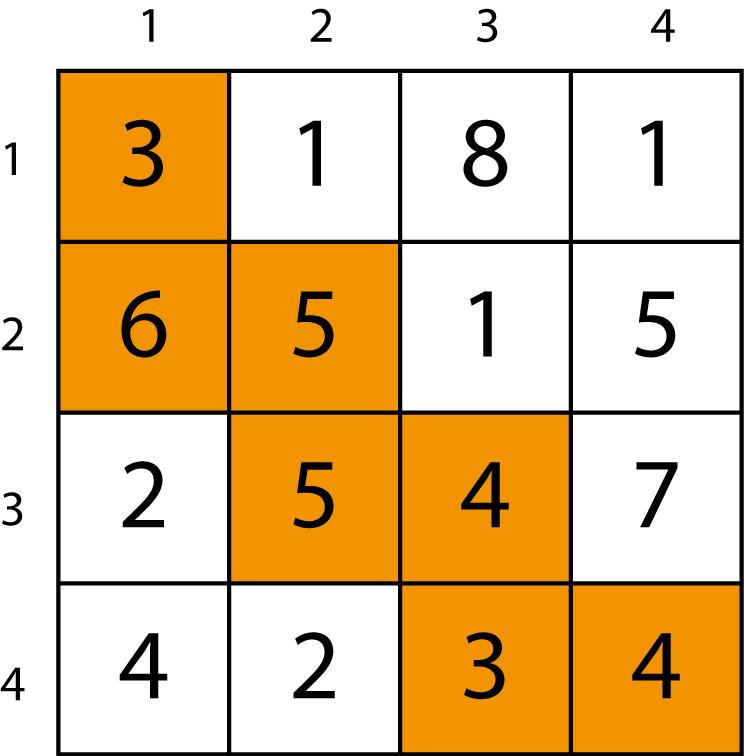
\includegraphics[width=1\textwidth]{img/3-2.png} 
  \caption*{\footnotesize Ejemplo con H=2. El costo del camino mínimo resultante es 1.}
  \label{fig:3-2}
\end{minipage}
\end{figure}

\newpage

\subsection{Formulación Recursiva}

Obtendremos la solución del problema usando un algoritmo de programación dinámica. Para eso, planteamos una formulación recursiva del problema. Sea la función $f$:

$f(i,j) = $ costo de un camino óptimo desde $ M_{1,1} $ hasta $ M{i,j}$

Entonces, la solución del problema está dada por $f(n,m)$. 
Se propone la siguiente recursión para calcular $f$:

\begin{equation} \label{formulacionRecursiva}
f(i,j) = min \left( 
	\begin{array}{lr}
    f(i-1, j) + Costo(M_{i-1,j} \rightarrow M_{i,j}), \\
	f(i,j-1) + Costo(M_{i,j-1} \rightarrow M_{i,j}) \\
     \end{array}
   \right)
\end{equation}  

con algunos casos particulares:

$f(1,1) = 0 $

$f(1,j) = f(1,j-1) + Costo(M_{1,j-1} \rightarrow M_{1,j})$

$f(i,1) = f(i-1,1) + Costo(M_{i-1,1} \rightarrow M_{i,1})$

\subsubsection{Demostración de Correctitud}

El caso base $f(1,1)$ es trivial, ya que no realizo ningún movimiento.

Dada cualquier otra posición $(i,j)$ de la matriz, el camino mínimo para llegar a ella tiene como última posición visitada o la casilla de su izquierda $(i, j-1)$ (si existe), o la casilla de arriba $(i-1, j)$ (si existe) por el enunciado del problema, ya que los únicos movimientos posibles son moverse hacia abajo o hacia la derecha.

Para demostrar que la función $f$ propuesta calcula el camino mínimo hasta una casilla cualquiera $M_{i,j}$ debemos ver que se cumple el \textbf{Principio de Optimalidad.} Es decir, que dado un camino óptimo desde $M_{1,1}$ hasta $M{i,j}$, $P_{i,j}$, entonces, el subcamino desde $M_{1,1}$ hasta el inmediato antecesor de $M_{i,j}$ ($P_{i-1,j}$ o $P{i,j-1}$) debe ser óptimo: 

Sea $P_{i,j}$ el camino óptimo desde $M_{1,1}$ $hasta M{i,j}$.
SPGE, puedo suponer que el inmediato antecesor de $M_{i,j}$ en $P$ es $M_{i, j-1}$. Supongamos que elsub camino hasta el antecesor de $M_{i,j}$ ($P_{i,j-1}$)  no es óptimo. Entonces, $\exists$ $P\prime_{i,j-1}$ tal que $Costo(P\prime_{i,j-1})$ $<$ $Costo(P_{i,j-1})$.

Pero entonces, puedo tomar el camino  $P\prime_{i,j-1}$ y de ahí moverme a la posición $M_{i,j}$. 
$Costo (P\prime_{i,j-1}) + Costo(M_{i-1,j} \rightarrow M_{i,j}) < Costo (P{i,j-1}) + Costo(M_{i-1,j} \rightarrow M_{i,j}) = Costo(P_{i,j})$
Pero esto es absurdo, ya que existiría un camino mejor que el óptimo hasta la posición $(i,j)$.

Como aplica el principio de optimalidad y sólo hay dos posibles antecesores para una determinada casilla $M_{i,j}$, para calcular el camino mínimo hasta una posición $(i,j)$ basta con tomar el mínimo entre las dos posibilidades, tomando el cuenta el costo de realizar el último movimiento. Es decir, el de menor costo sumando el costo de dar el último movimiento.

Para los casos borde de la matriz, en la primera columna y en la primera fila, donde sólo tengo un sólo posible antecesor (el inmediato de abajo y el inmediato de la izquierda respectivamente), el camino mínimo entonces es el camino mínimo hasta el único antecesor más el último movimiento. $\qed$

\subsection{Pseudocódigo}

Se presenta a continuación el pseudocódigo del algoritmo propuesto que resuelve el problema. El algoritmo calcula la función recursiva definida anteriormente para todas las posiciones posibles de la matriz, es decir, el costo mínimo para alcanzar cada una de esas posiciones, guardando junto con el resultado la lista de movimientos para llegar a  cada una de ellas. 
Como se explica en la sección anterior, el costo para llegar a una posición determinada $(i,j)$ depende solamente del costo para llegar a las posiciones $(i-1, j)$ y $(i,j-1)$. En los casos particulares de casilleros que se encuentran en la primera columna o en la primera fila de la matriz, los costos dependen solamente del costo para llegar al casillero de arriba o de la izquierda respectivamente. Esto permite implementar un algoritmo \textbf{bottom-up}, es decir, podemos definir un orden determinado para calcular los resultados parciales iterativamente, evitando el overhead que resultaría de implementar la función recursivamente (top-down). Entonces, resolvemos primero los subproblemas más chicos y luego los subproblemas más grandes, guardando los resultados en un diccionario. El orden propuesto es resolver por filas, empezando por la fila 1 y terminando por la fila N, de izquierda a derecha:

\begin{figure}[H]
 \centering
	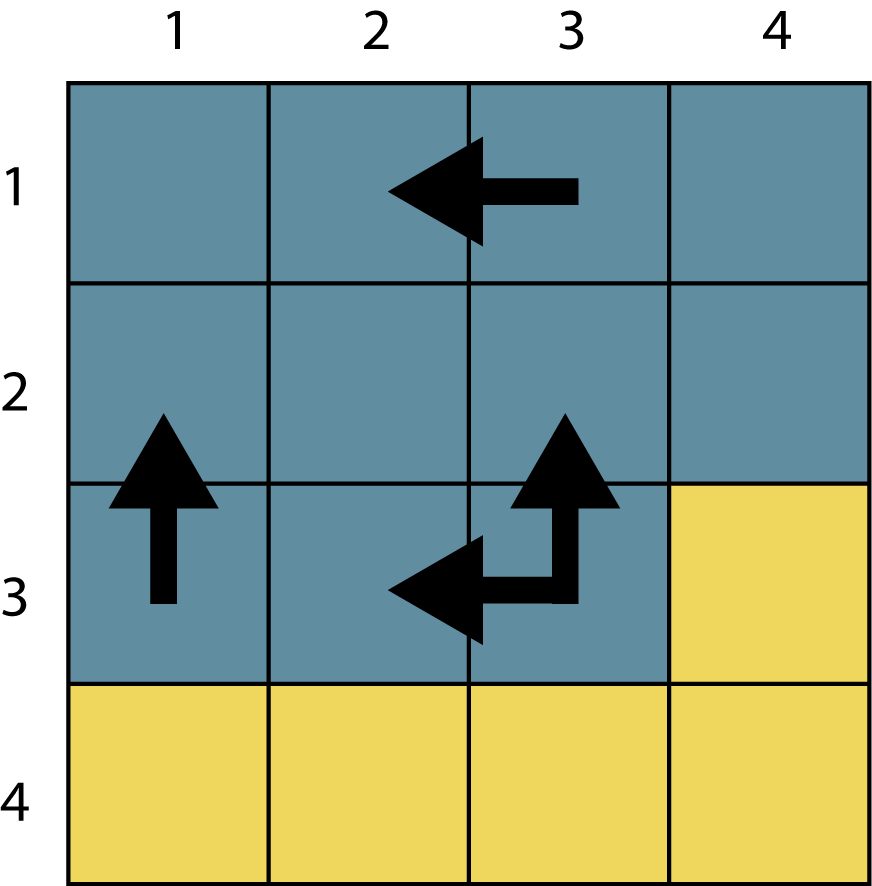
\includegraphics[width=0.4\textwidth]{img/3-3.png}
	\caption{\footnotesize Dependencias entre subproblemas.}
	\label{fig:3-3}
\end{figure}

Como se ve en la figura \ref{fig:3-3}, al resolver los subproblemas en este orden 
se respetan las dependencias entre los mismos, ya que al resolver uno ya se tienen calculados los resultados de los subproblemas correspondientes al casillero de la izquierda y al casillero por encima del mismo.

Para representar el diccionario donde se guardan los resultados de los subproblemas, utilizamos una matriz de triplas de tamaño $n \times m$, donde cada tripla es de tipo a : <\texttt{int}: $Altura$, \texttt{int}: $CostoM\acute{\imath}nimo$, \texttt{char}: $Movmimiento$>. Los campos corresponden a:
\begin{itemize}
\item la $Altura$ de cada casillero, ingresada por parámetro
\item el $CostoM\acute{\imath}nimo$ para llegar a dicha casilla, que va calculando el algoritmo y guardando en la matriz
\item el último $Movimiento$ para llegar a dicha casilla por el camino de costo mínimo, donde $X$ corresponde a un movimiento de tipo $M_{i,j} \rightarrow M_{i+1,j}$, y $Y$ corresponde a un movimiento de tipo $M_{i,j} \rightarrow M_{i,j+1}$.
\end{itemize}
Basta con guardar el último movimiento, ya que para rearmar la lista de movimientos entera, al final podemos recorrer el camino de costo mínimo de casilleros desde la posición ($n,m$) usando el último movimiento de cada uno de ellos.

\begin{algorithm}[H]
  \begin{algorithmic}[1]
  \caption{Pseudocódigo del \texttt{main}}
  \label{algo:3-1}
  \Procedure{main}{}
 	\State $n, m, h \gets INPUT$
 	\State \texttt{vector<vector<Casilla>\null>} $Tablero$ 
 	\Comment creo matriz de $n \times m$
 	\Comment $\Theta(n\times m)$
 	\State \texttt{InicializarAlturas}($Tablero$) 
 	\Comment completo las casillas con sus respectivas alturas, $\Theta(n\times m)$
	\State \texttt{int} $res \gets$ \texttt{solve}($Tablero,n,m,h$)
	\Comment $\Theta(n\times m)$
	\State \texttt{list<char>} $camino$
	\Comment $O(1)$
	\State \texttt{int} $i \gets n-1$
	\Comment $O(1)$
	\State \texttt{int} $j \gets m-1$
	\Comment $O(1)$
	\While {$!(i == 0\ \&\&\ j == 0)$}
	\Comment $\Theta(n+m)$
		\State \texttt{const char} $mov \gets Tablero[i][j]\{Movimiento\}$
		\Comment $O(1)$
		\State $camino$.\texttt{pushfront}$(mov)$
		\Comment $O(1)$
		\State IF $mov == Y$ THEN $j--$ ELSE $i--$ FI
		\Comment $O(1)$
	\EndWhile
	\State Imprimir ($res$, $camino$)
	\Comment $\Theta(n+m)$
    \EndProcedure
  \end{algorithmic}
\end{algorithm}

  
\begin{algorithm}[H]
  \begin{algorithmic}[1]
  \caption{Pseudocódigo de función \texttt{solve}}
  \label{algo:3-2}
    \Procedure{solve}{\texttt{vector<vector<Casilla>\null>} $\&t$, \texttt{int} $n$, $m$, $h$} $\rightarrow$ \texttt{int} $CostoM\acute{\imath}nimo$
		\State $t[0][0]\{CostoM\acute{\imath}nimo\} \gets 0$
		\Comment $\Theta(1)$
		\For {\texttt{int} $j$ desde $1$ hasta $m-1$}
		\Comment $\Theta(m)$
			\State $t[0][j]\{CostoM\acute{\imath}nimo\} \gets costoColumna(t,h,0,j)$
			\Comment $\Theta(1)$
			\State $t[0][j]\{Movimiento\} \gets $'$Y$'$ $
			\Comment $\Theta(1)$
		\EndFor
		\For { \texttt{int} $i$ desde $1$ hasta $n-1$ }
		\Comment $\Theta(n)$
			\State $t[i][0]\{CostoM\acute{\imath}nimo\} \gets costoFila(t,h,i,0)$
			\Comment $\Theta(1)$
			\State $t[i][0]\{Movimiento\} \gets $'$X$'$ $
			\Comment $\Theta(1)$
		\EndFor
		\For {$i$ desde $1$ hasta $n-1$}
		\Comment $\Theta(n \times m)$
			\For {$j$ desde $1$ hasta $m-1$}
				\State $t[i][j]\{costoM\acute{\imath}nimo\} \gets min\{costoFila(t,h,i,j), costoColumna(t,h,i,j)\} \ \  \Theta(1)$
				\If {$t[i][j]\{CostoM\acute{\imath}nimo\} == costoFila(t,h,i,j)$}
				\Comment $\Theta(1)$
					\State $t[i][j]\{Movimiento\} \gets $'$X$'$ $ 
					\Comment $\Theta(1)$
				\Else
					\State $t[i][j]\{Movimiento\} \gets $'$Y$'$ $
					\Comment $\Theta(1)$
				\EndIf
			\EndFor
		\EndFor
	\State \texttt{return} $t[n-1][m-1]\{CostoM\acute{\imath}nimo\}$
	\Comment $\Theta(1)$
	\EndProcedure
	\end{algorithmic}
\end{algorithm}

donde:
\begin{itemize}
\item \texttt{costoFila}($t,h,i,j$) = $t[i-1][j]\{CostoM\acute{\imath}nimo\}\ + \ Costo(M_{i,j} \rightarrow M_{i+1,j})$
\item \texttt{costoColumna}($t,h,i,j$) = $t[i][j-1]\{CostoM\acute{\imath}nimo\}\ + \ Costo(M_{i,j} \rightarrow M_{i,j+1})$
\end{itemize}
Ambas pueden ser calculadas en $O(1)$.

\subsection{Complejidad del algoritmo}

La complejidad de los algoritmos se puede deducir fácilmente de los pseudocódigos \ref{algo:3-1} y \ref{algo:3-2}. La función \texttt{solve} que resuelve los subproblemas y los guarda en la matriz, es $\Theta(n\times m)$, debido a que siempre tendrá que resolver $n\times m$ subproblemas para obtener el resultado. Luego, recuperar e imprimir la lista de movimientos es $\Theta(n+m)$, ya que un camino desde la posición $(1,1)$ hasta la posición $(N,M)$ realizado con los movimientos descriptos en secciones anteriores siempre tiene un largo de $n+m$ casilleros. Como $\Theta(n+m) \ + \Theta(n\times m) + \Theta(1) = \Theta(n\times m)$, concluimos que la complejidad del algoritmo es \textbf{$\Theta(n\times m)$}.

\subsection{Performance del algoritmo}


Como dijimos antes, la complejidad del algoritmo es siempre $\Theta(n m)$, sin distinción entre casos, por lo que el análisis de performance es simple.

Primero veamos que, en la práctica, la complejidad del algoritmo es efectivamente $\Theta(n \log n)$.

\begin{figure}[H]
 \centering
	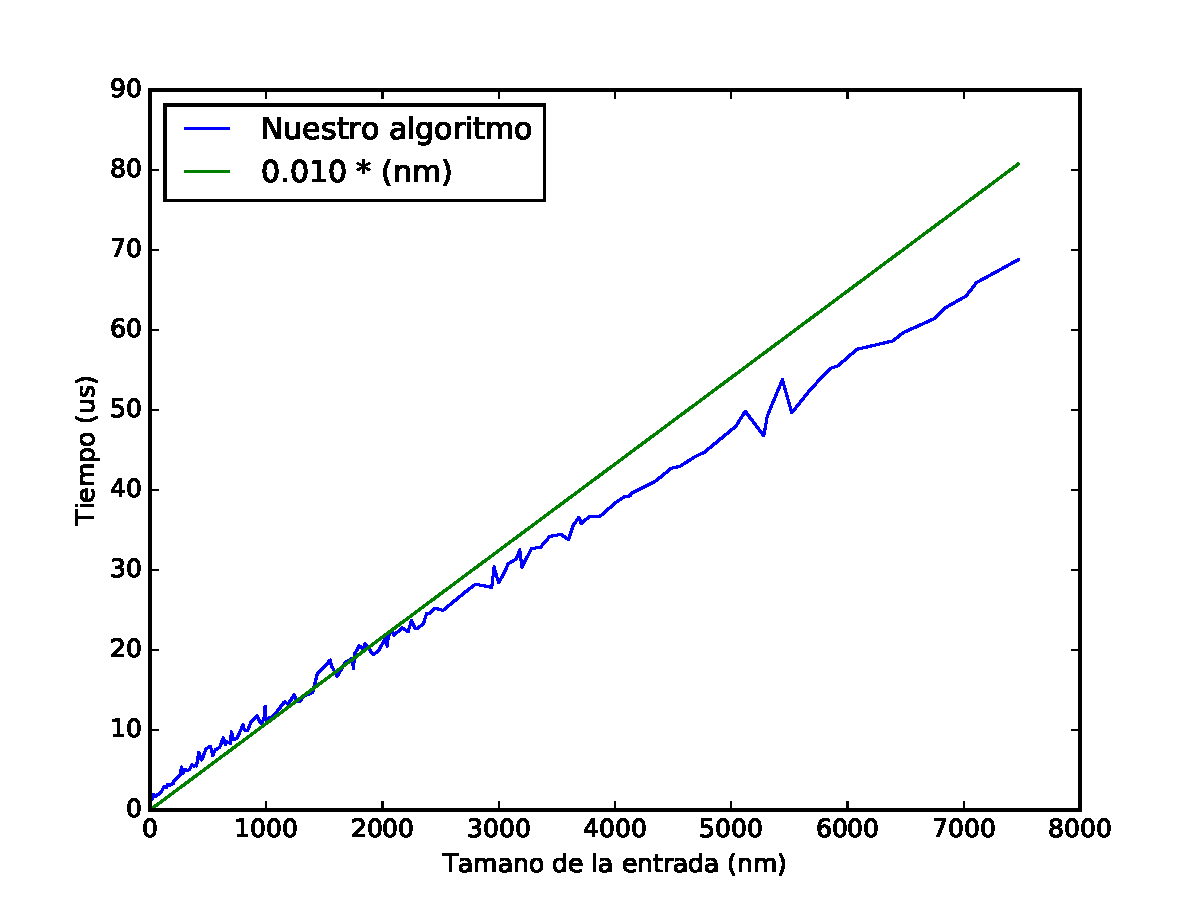
\includegraphics[width=0.8\textwidth]{img/exp/problema3-promedio.pdf}
	\caption{\footnotesize Tiempo que toma el algoritmo en $\mu$s para una entrada de tamaño $mn$.}
	\label{fig:problema3-promedio}
\end{figure}

En esta imagen se ve que se comporta como debe. Sin embargo, al igual que en los problemas anteriores, para confirmarlo totalmente, realizamos el gráfico de $\frac{T(nm)}{nm}$, dado que si esta función tiene a una constante cuando $nm \to \infty$, habremos confirmado experimentalmente que la complejidad del algoritmo es de $\Theta(n m)$.

\begin{figure}[H]
 \centering
	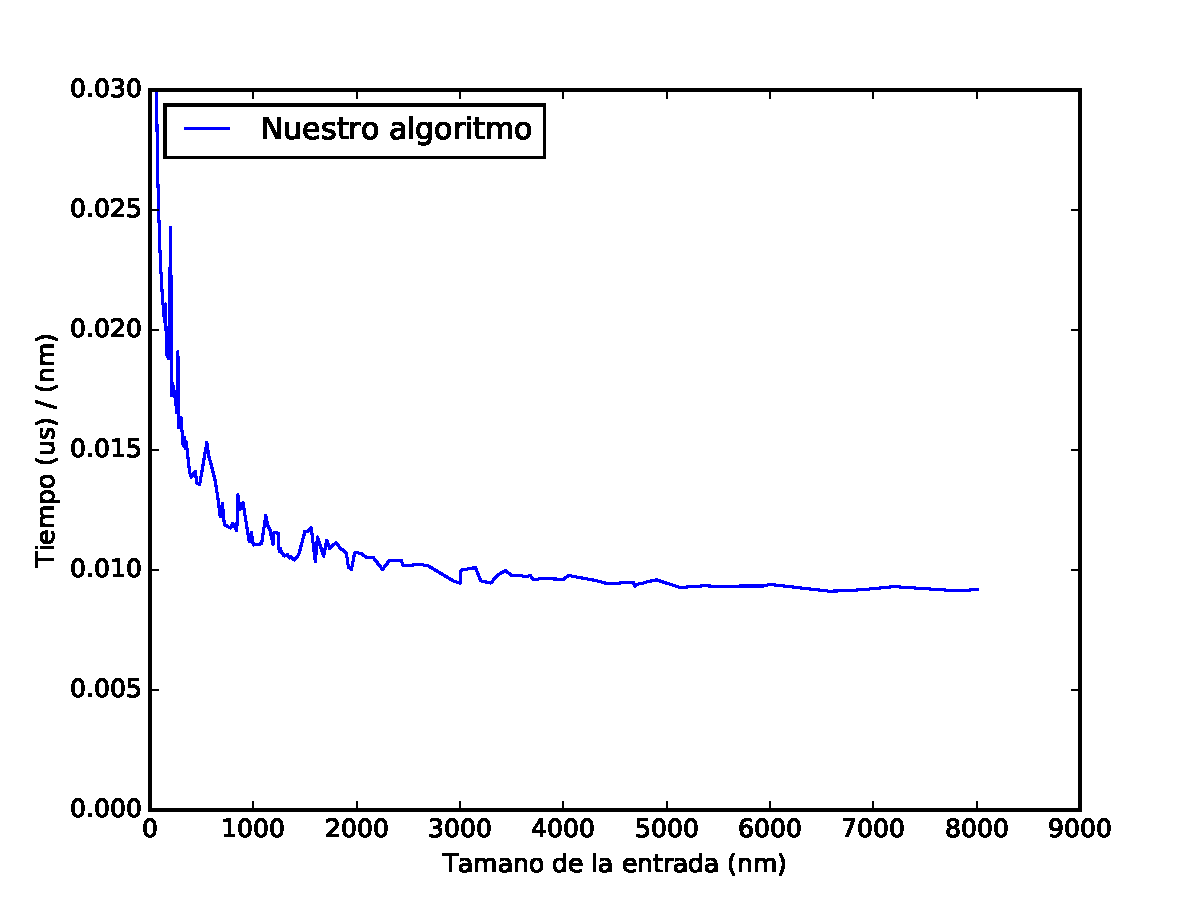
\includegraphics[width=0.8\textwidth]{img/exp/problema3-promedio2.pdf}
	\caption{\footnotesize Tiempo que toma el algoritmo en $\mu$s dividido $mn$ para una entrada de tamaño $mn$.}
	\label{fig:problema3-promedio2}
\end{figure}


\subsubsection{M\'etodo de experimentación}

